\documentclass{beamer}
\usetheme{Warsaw}

\usepackage[utf8]{inputenc}
\usepackage{fancybox}
\usepackage{multimedia} 
\usepackage{subfig}
\usepackage{amsmath}

\usepackage[all]{xy}
\begin{document}


\title[Computergrafik] % (optional, only for long titles)
{Computergrafik

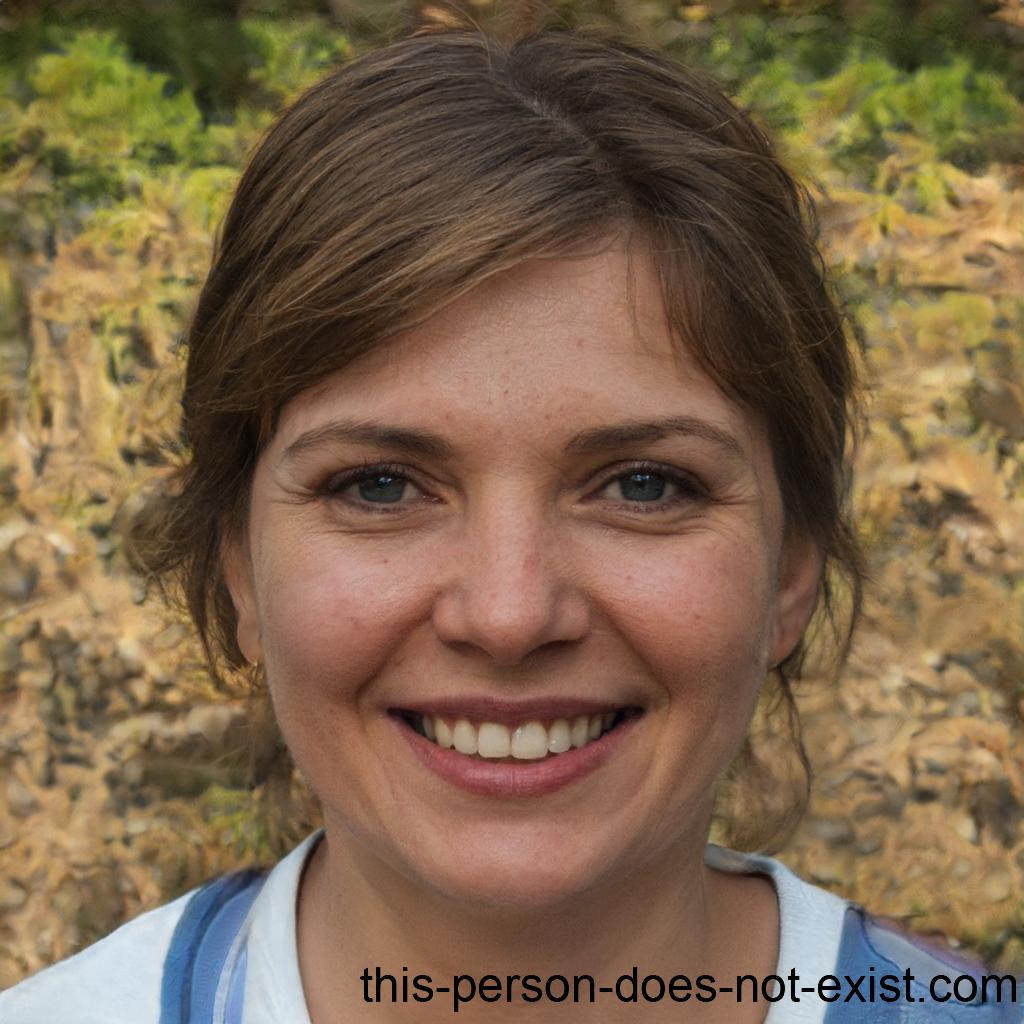
\includegraphics[scale=0.36]{images/person}
}
\subtitle{}
\author[Dr. Johannes Riesterer] % (optional, for multiple authors)
{Dr.  rer. nat. Johannes Riesterer}

\date[KPT 2004] % (optional)
{}

\subject{Computergrafik}


\begin{frame}
    \frametitle{Generative Modelle}
\framesubtitle{}
\begin{block}{Diese Person existiert nicht! https://this-person-does-not-exist.com/de}
    \center
    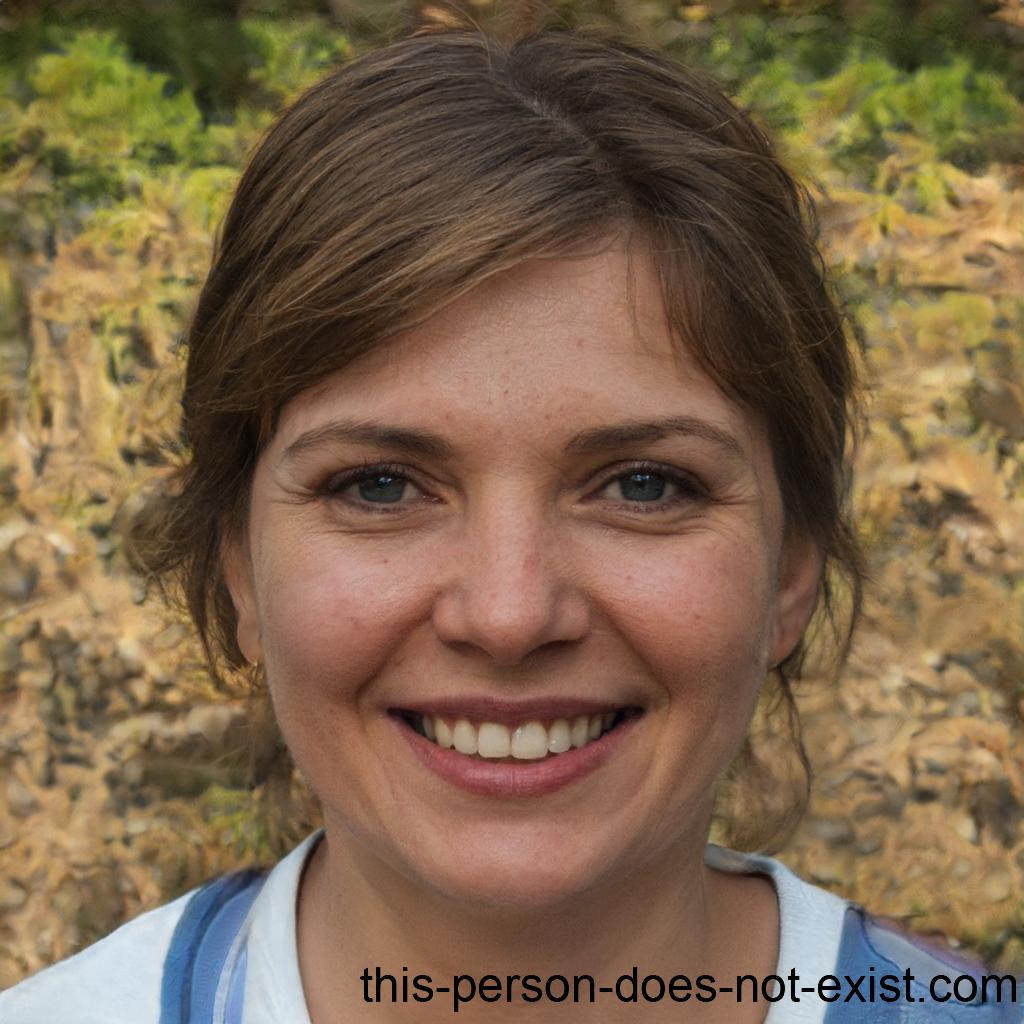
\includegraphics[scale=0.25]{images/person}
\end{block}
\end{frame}


\begin{frame}
    \frametitle{Generative AI}
\framesubtitle{}
\begin{block}{Generative AI (Wiki)}
    Generative künstliche Intelligenz (auch generative KI oder GenAI) bezeichnet künstliche Intelligenz, 
    die in der Lage ist, Texte, Bilder oder andere Medien mithilfe generativer Modelle zu erzeugen. Generative KI-Modelle lernen die Muster und Struktur ihrer Eingabedaten während des Trainings und erzeugen anschließend neue Daten mit ähnlichen Merkmalen.
\end{block}
\begin{block}{Generative AI (ChatGPT (Selbst eine generative AI))}
 
Ein generatives Modell in der künstlichen Intelligenz (KI) ist ein Typ von Modell, 
das darauf abzielt, neue Daten zu erstellen, die ähnlich zu den Trainingsdaten sind, 
mit denen es trainiert wurde. Im Gegensatz zu diskriminativen Modellen, 
die darauf ausgelegt sind, zwischen verschiedenen Klassen oder Kategorien zu unterscheiden, 
versucht ein generatives Modell, 
die Verteilung der Trainingsdaten zu erfassen, um neue Daten zu generieren.
\end{block}
\end{frame}

\begin{frame}
    \frametitle{Generative AI}
\framesubtitle{}
\begin{block}{Generative AI}
    Einsatzgebiete in der Computergrafik:
  \begin{itemize}
    \item Generierung von (teilbereichen in) Bildern.
    \item Konstruktion von 2D und 3D Modellen.
    \item Upsampling von Bildern auf eine höhere Auflösung.
    \item Filter (Endrauschen bei Pathtracing).
  \end{itemize}
\end{block}
\end{frame}


\begin{frame}
    \frametitle{Angewandte Mathematik}
\framesubtitle{Backpropagation}
    \begin{block}{Backpropagation}
Das Gradientenverfahren angewendet auf eine Lossfunktion eines neuronalen Netzes wird als Backpropagation bezeichnet.
Gegeben ist ein neuronales Netz $f : \Omega \times \mathbb{R}^n \to \mathbb{R}^m$, 
und ein  Datensatz $D : = \{ (x_i, y_i) \}$ mit $x_i \in \mathbb{R}^n, y_i \in \mathbb{R}^m$. Finde Gewichte Omega, so dass Lossfunktion
\begin{align*}
L_D  : \Omega \subset \mathbb{R}^n \to \mathbb{R} 
\end{align*}
minimal wird. Zum Beispiel $$L_D(\omega) := \sum_{(x_i,y_i) \in D} (f(\omega, x_i) - y_i)^2$$.

\end{block}
 \end{frame}


 \begin{frame}
    \frametitle{Mehrdimensionale Differentialrechnung}
\framesubtitle{Differenzierbarkeit}
    \begin{block}{Gradient}

Der Vektor 
$$\nabla f (a) := \begin{pmatrix}  \frac{\partial f(a)}{\partial x_1} \\  \vdots \\ \frac{\partial f(a)}{\partial x_n}  \end{pmatrix}$$
wird als Gradient bezeichnet. Es ist $df(a) \cdot h = \langle \nabla f (a) , h \rangle$.
\end{block}
\begin{figure}[H]
      \centering
    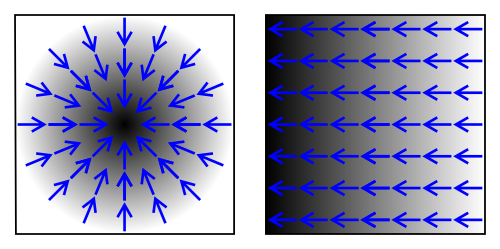
\includegraphics[width=0.7\textwidth]{images/Gradient}
      \caption{Quelle: Wikipedia: https://commons.wikimedia.org/wiki/File:Gradient2.svg}
\end{figure}


 \end{frame}

\begin{frame}
    \frametitle{Angewandte Mathematik}
\framesubtitle{Backpropagation}
 \begin{figure}[!tbp]
  \centering
  \begin{minipage}[b]{0.45\textwidth}
    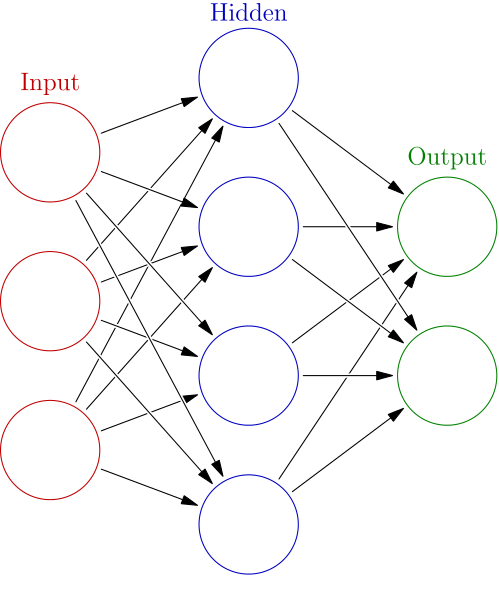
\includegraphics[width=0.6\textwidth]{images/499px-Colored_neural_network}
    \caption{}
  \end{minipage}
  \hfill
  \begin{minipage}[b]{0.45\textwidth}
    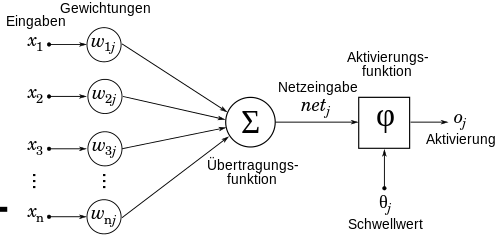
\includegraphics[width=1.0\textwidth]{images/500px-NeuronModel_deutsch}
    \caption{}
  \end{minipage}
\end{figure}
 \end{frame}


\begin{frame}
    \frametitle{Angewandte Mathematik}
\framesubtitle{Gradientenverfahren}
    \begin{block}{Gradientenverfahren}
Wie kann man Minima einer  differenzierbaren Abbildung $f: \mathbb{R}^n \to \mathbb{R}$ finden? 
 
\end{block}

    \begin{block}{Gradientenverfahren}
\begin{itemize}
\item An jedem Punkt $x_k \in  \mathbb{R}^n$ zeigt der negative Gradient  $d_k := -\nabla f (x_k)$ in die steilste Abstiegsrichtung.
\item Für hinreichend kleines $\alpha_k$ folgt mit Satz über die lokale Linearisierung:
$f(x_{k+1}) = f (x_k + \alpha_k d_k) =  f(x_k) + \alpha_k df(x_k)d_k + R( \alpha_k dk)$
\item  Setze $x_{k+1} = x_k + \alpha_k d_k$ 
\item Es gilt $f(x_{k+1}) \leq f(x_k)$, falls $\nabla f(x_k) \neq 0$
\item  Falls die folge $f(x_k)$ beschränkt ist, so ist  dieser Fixpunkt $x^*$ ein Minimum, da $\nabla f(x^*) = 0$ gelten muss.  
\end{itemize}

\end{block}
 \end{frame}



\begin{frame}
    \frametitle{Angewandte Mathematik}
\framesubtitle{Gradientenverfahren}
\begin{figure}[H]
      \centering
    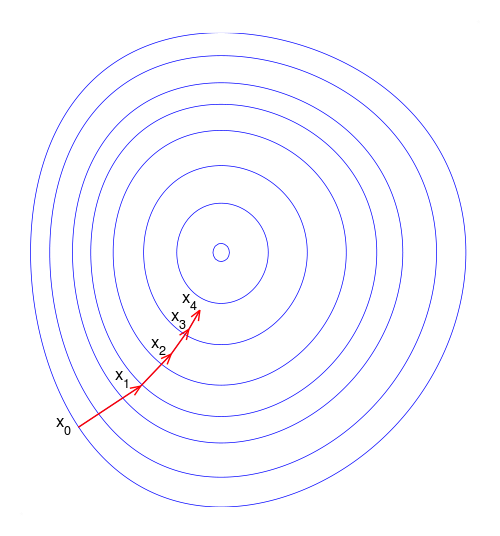
\includegraphics[width=0.5\textwidth]{images/Gradient_descent}
      \caption{Quelle: Wikipedia}
\end{figure}

 \end{frame}




\begin{frame}
    \frametitle{Angewandte Mathematik}
\framesubtitle{Gradientenverfahren}
    \begin{block}{Höhenlinien}
Sei  $f: \mathbb{R}^n \to \mathbb{R}$  eine differenzierbare Funktion. Eine Kurve $\gamma : I \to \mathbb{R}^n$, auf der $f$ konstant ist, also 
$f(\gamma(t)) = c$ für ein festes $c \in \mathbb{R}$ gilt, heißt Höhenlinie.
\end{block}

\begin{figure}[H]
      \centering
    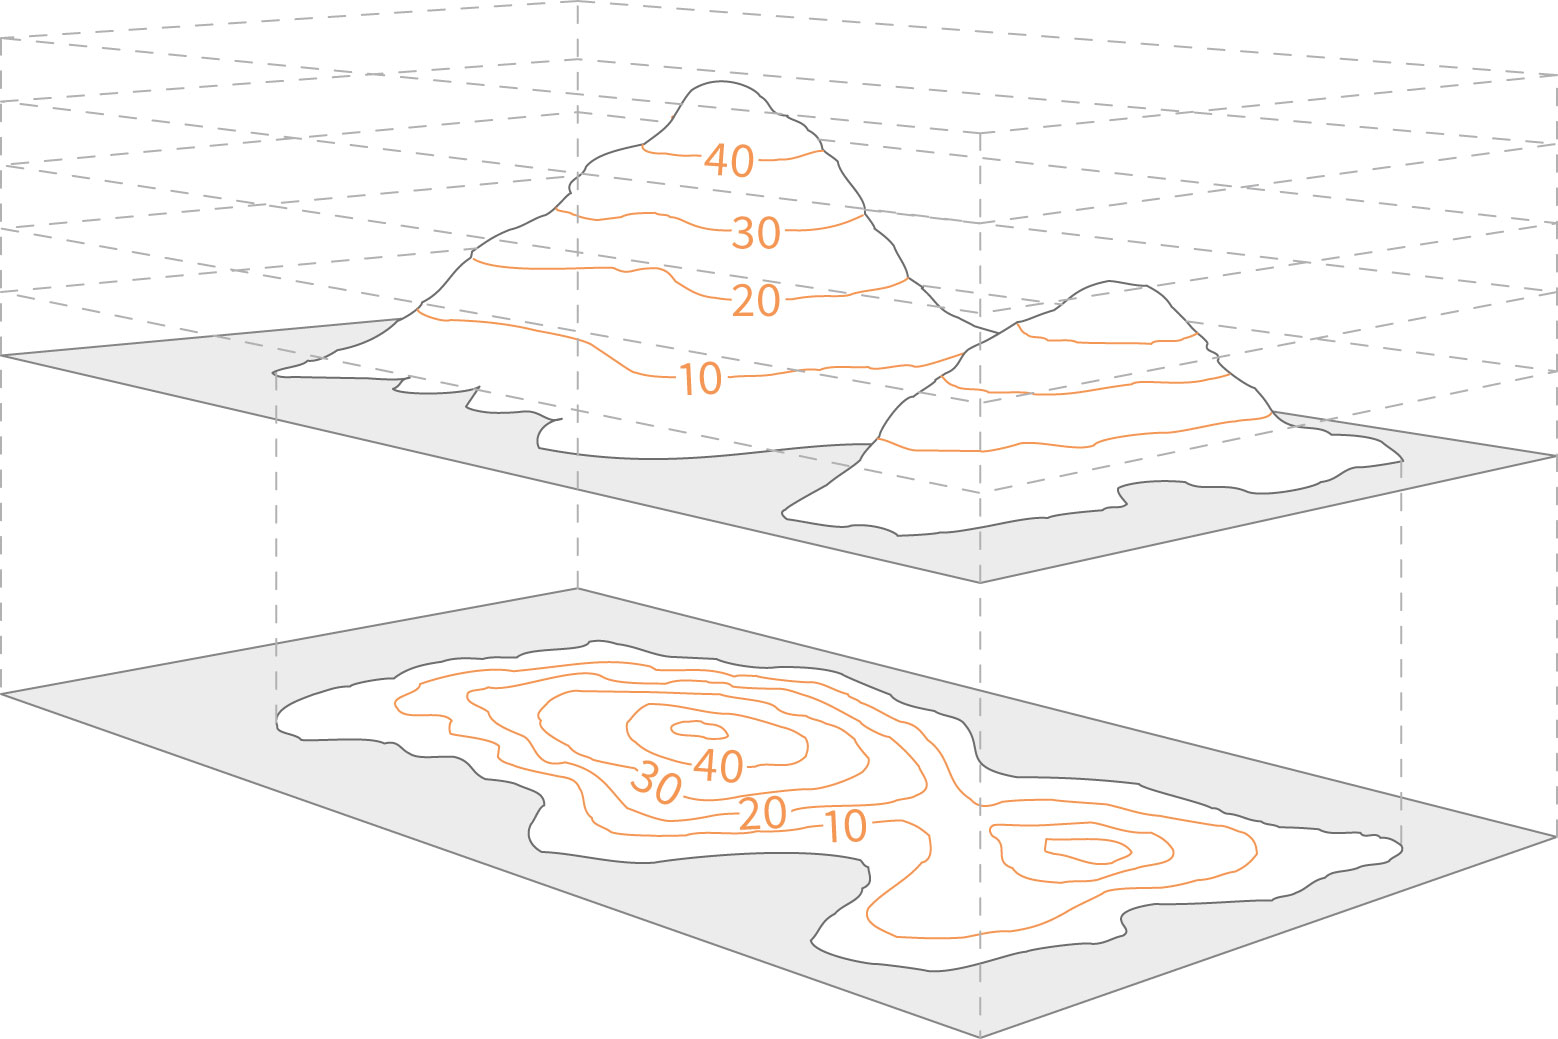
\includegraphics[width=0.5\textwidth]{images/Contours-and-relief}
      \caption{Quelle: https://getoutside.ordnancesurvey.co.uk/guides/understanding-map-contour-lines-for-beginners/}
\end{figure}

 \end{frame}


\begin{frame}
    \frametitle{Angewandte Mathematik}
\framesubtitle{Gradientenverfahren}
    \begin{block}{Höhenlinien}
Der Gradient steht senkrecht auf  Höhenlinien. 
\end{block}
  

 \end{frame}




\begin{frame}
    \frametitle{Angewandte Mathematik}
\framesubtitle{Backpropagation}
    \begin{block}{Backpropagation}
\begin{itemize}
\item  Initialisiere $k:=0$ und zufällige Gewichte $w_0$.
\item \pause Initialisiere Genauigkeit $\epsilon > 0$
\item \pause   \text{While } {$|| \nabla L_D(\omega) || > \epsilon$}  
\item \pause Bestimme $\alpha_k$  mit $ L_D(\omega_k + \alpha d_k) =  L_D(\omega_k) + \alpha_k d L_D(\omega_k)d_k + R( \alpha_k dk)$ 
\item \pause  Setze $\omega_{k+1} := \omega_k  + \alpha_k d_k$. 
\item \pause $k \leftarrow k+1$
\end{itemize}
\end{block}
 \end{frame}

\begin{frame}
    \frametitle{Angewandte Mathematik}
\framesubtitle{Backpropagation}
    \begin{block}{Mini Batch}
\begin{itemize}
\item   Datensatz $D$ sehr groß (Big Data)
\item \pause Berechnung des Gradienten der Lossfunktion entsprechend aufwendig. 
\item \pause Wende Backpropagation auf Teilräume $D' \subset D$ an (Minibatch).
\item \pause $\#D' = 1$ stochastischer Gradientenabstieg.
\end{itemize}

\end{block}
 \end{frame}



\begin{frame}
    \frametitle{Angewandte Mathematik}
\framesubtitle{Minibatch}
\begin{figure}[H]
      \centering
    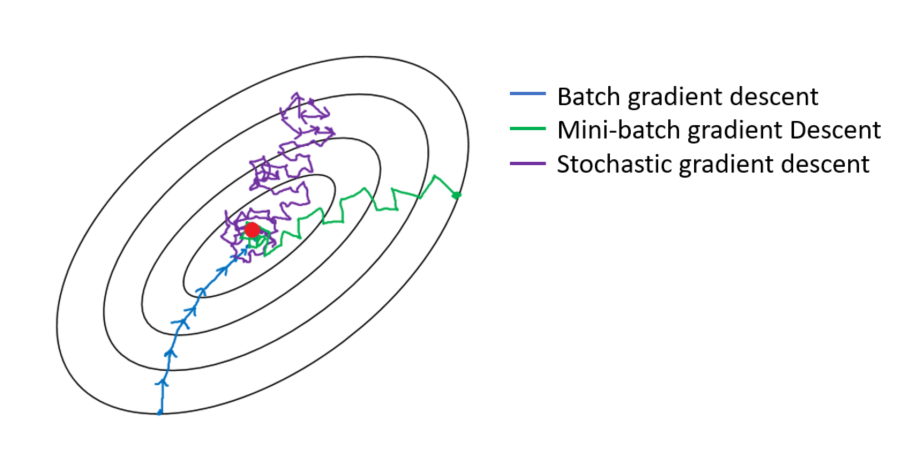
\includegraphics[width=1.0\textwidth]{images/batchgradient}
      \caption{Quelle: https://towardsdatascience.com/batch-mini-batch-stochastic-gradient-descent-7a62ecba642a}
\end{figure}

 \end{frame}



\begin{frame}
    \frametitle{Angewandte Mathematik}
\framesubtitle{Backpropagation}
    \begin{block}{Backpropagation}
\begin{itemize}
\item  Initialisiere $k:=0$ und zufällige Gewichte $w_0$.
\item \pause Initialisiere Genauigkeit $\epsilon > 0$
\item \pause Wähle Teilmenge $D_0' \subset D$
\item \pause   \text{While } {$|| \nabla L_{D_k'}(\omega) || > \epsilon$}  
\item \pause Bestimme $\alpha_k$  mit $ L_{D_k'}(\omega_k + \alpha d_k) =  L_{D_k'}(\omega_k) + \alpha_k d L_{D_k'}(\omega_k)d_k + R( \alpha_k dk)$ 
\item \pause  Setze $\omega_{k+1} := \omega_k  + \alpha_k d_k$. 
\item \pause Wähle neue Teilmenge $D'_{k +1} \subset D$.
\item \pause $k \leftarrow k+1$
\end{itemize}
\end{block}
 \end{frame}


\begin{frame}
    \frametitle{Angewandte Mathematik}
\framesubtitle{Automatisches Ableiten}
\begin{figure}[H]
      \centering
    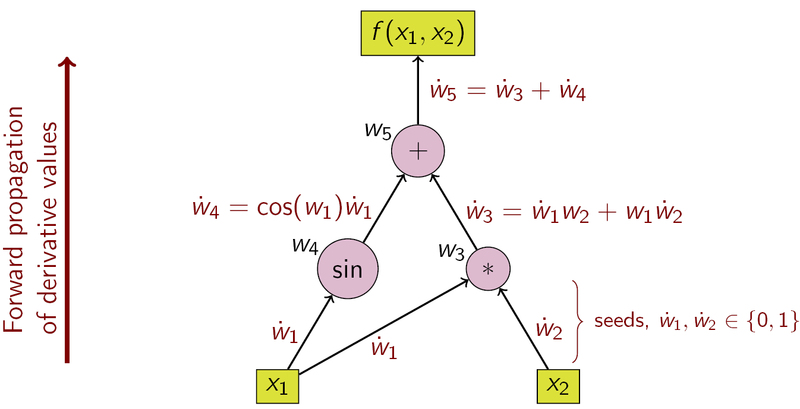
\includegraphics[width=0.8\textwidth]{images/ad.png}
      \caption{Quelle: Wikipedia}
\end{figure}

\href{https://pytorch.org/tutorials/beginner/blitz/autograd_tutorial.html}{Automatisches Ableiten  in Pytorch}

\href{https://jax.readthedocs.io/en/latest/notebooks/quickstart.html}{Automatisches Ableiten  in JAX}

 \end{frame}



\begin{frame}
    \frametitle{Generative Modelle}
\framesubtitle{}
\begin{block}{Autoencoder}
    \center
    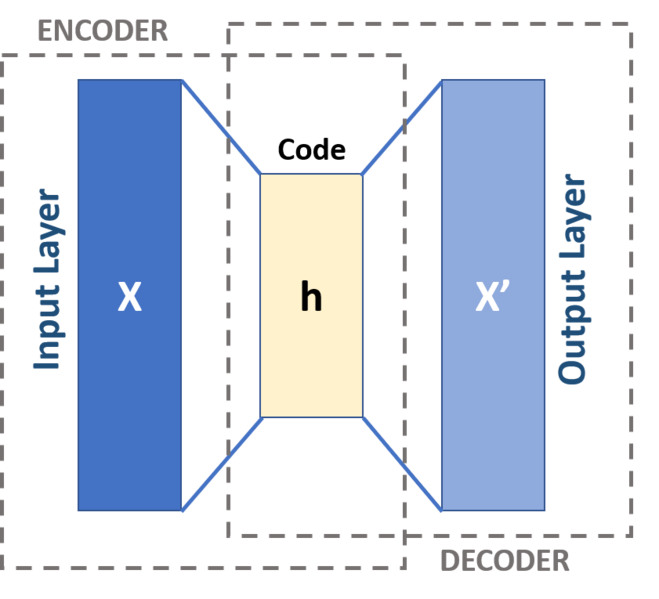
\includegraphics[scale=0.35]{images/autoencoder}
\end{block}
\begin{block}{Autoencoder}
    \center
    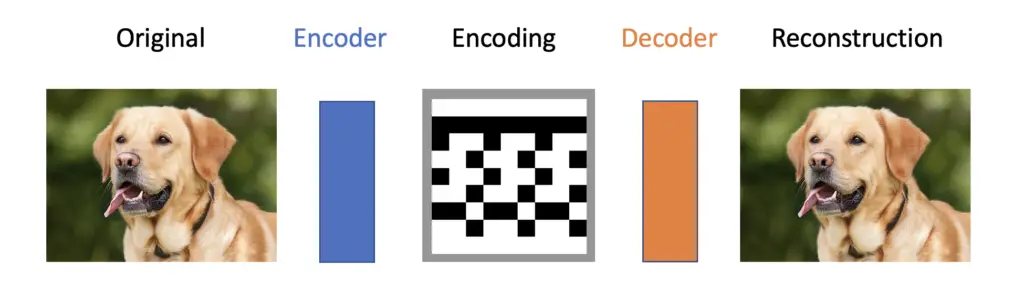
\includegraphics[scale=0.25]{images/autoencoder_train}
\end{block}
\end{frame}



\begin{frame}
    \frametitle{Generative Modelle}
\framesubtitle{}
    \begin{block}{GAN Architektur}
\begin{figure}[H]
    \centering
    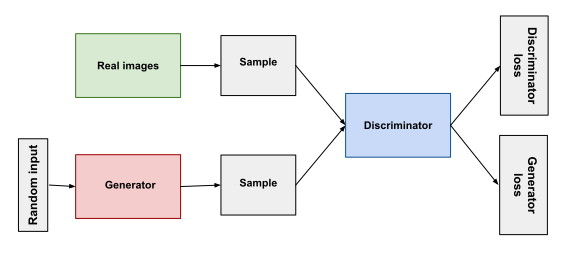
\includegraphics[width=0.6\textwidth]{images/gan_diagram}
\end{figure}
\end{block}
\begin{block}{Generator \& Discriminator}
    \begin{figure}[H]
        \centering
        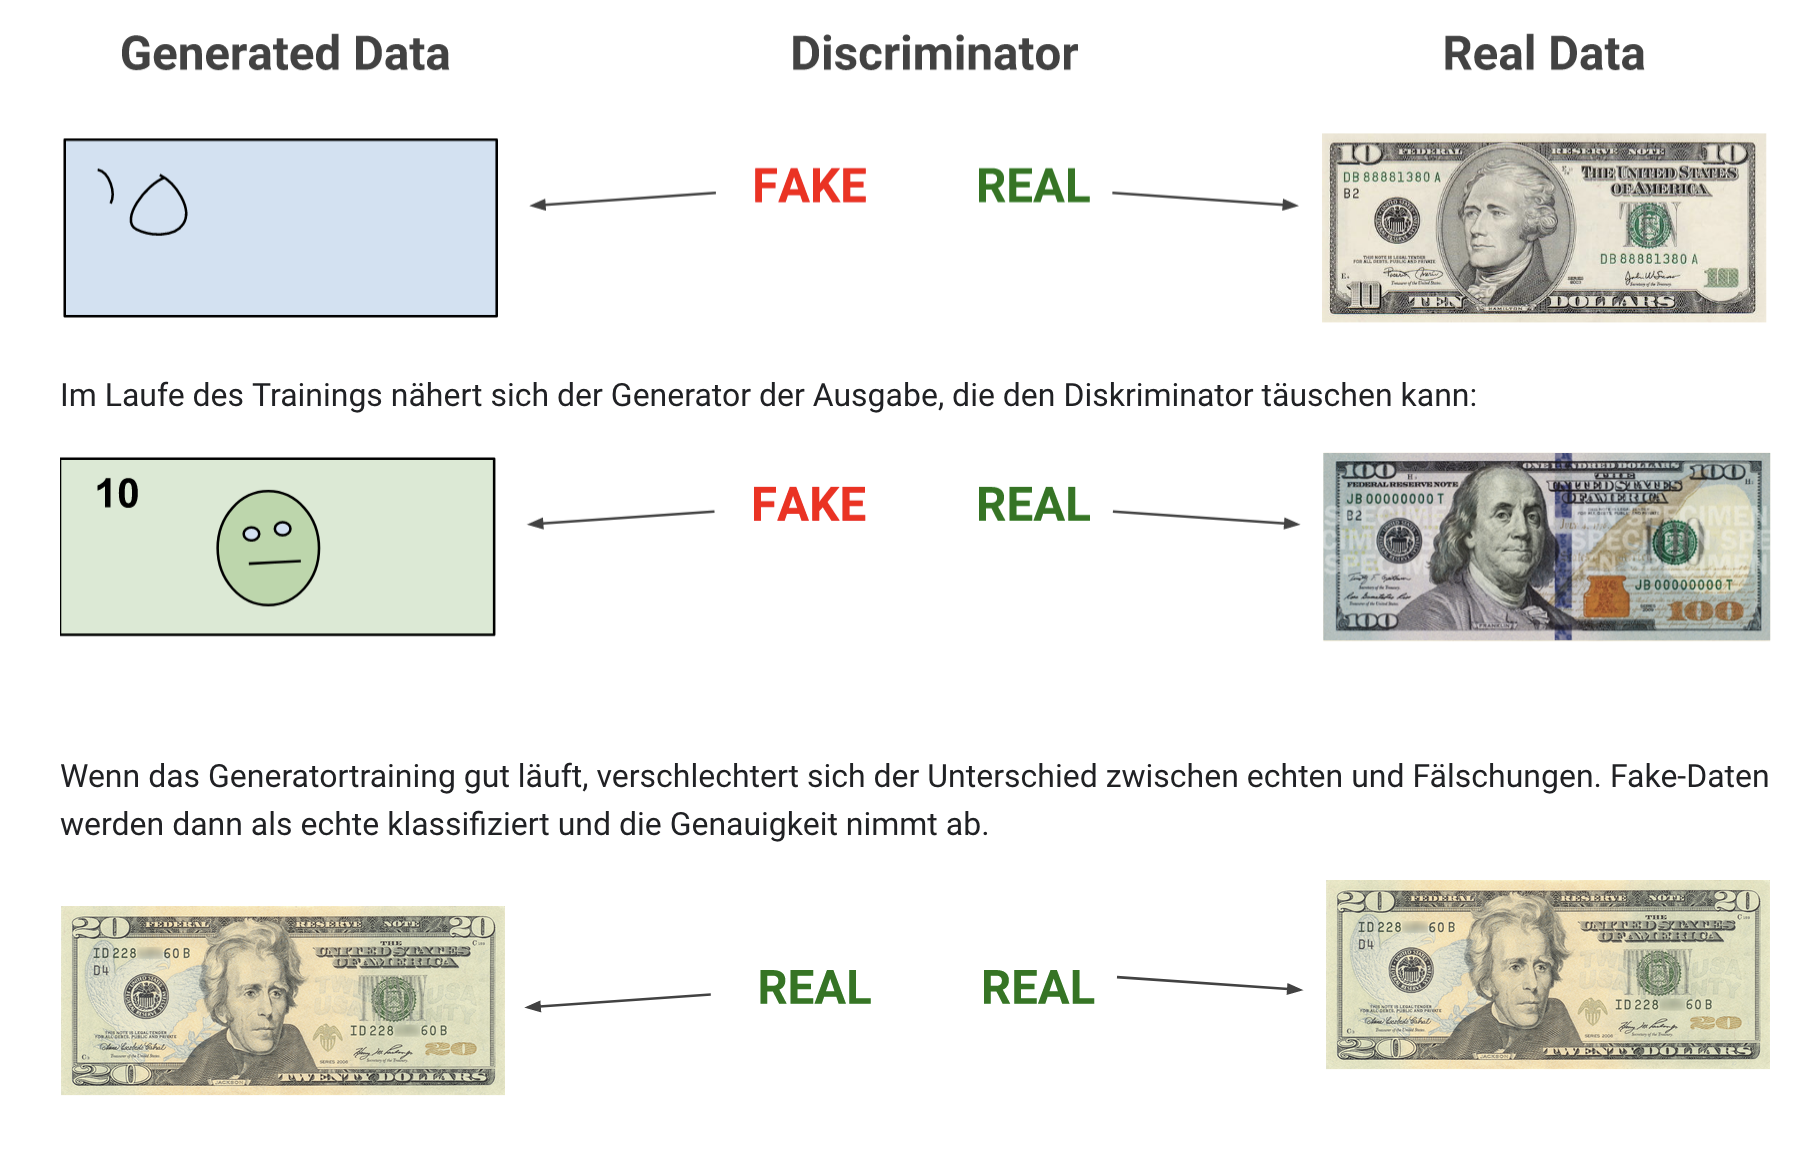
\includegraphics[width=0.45\textwidth]{images/gan_images}
    \end{figure}
    \end{block}
\end{frame}


\begin{frame}
    \frametitle{Generative Modelle}
\framesubtitle{}
    \begin{block}{Training Discriminator}
\begin{figure}[H]
    \centering
    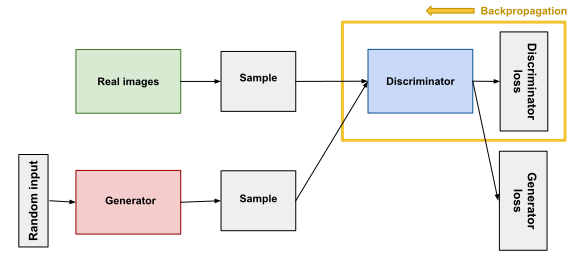
\includegraphics[width=0.55\textwidth]{images/gan_diagram_discriminator}
\end{figure}
\end{block}
\begin{block}{Training Generator}
    \begin{figure}[H]
        \centering
        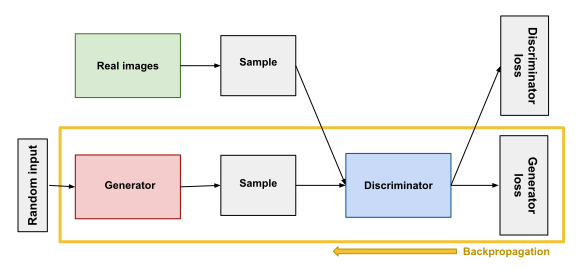
\includegraphics[width=0.55\textwidth]{images/gan_diagram_generator}
    \end{figure}
    \end{block}
\end{frame}


\end{document}
